\section{Monitor}
I semafori sono spesso utilizzare per sincronizzare l'utilizzo delle risorse, tuttavia il loro utilizzo incorretto può generare errori difficili da individuare.

\spacer
Un monitor è una struttura di più alto livello che contiene una serie di procedure e dei dati (condivisi tra i processi).
La caratteristica di un monitor è che al suo interno un solo processo per volta può essere attivo.

\begin{minted}{java}
monitor monitor_name {
    /* dichiarazioni delle variabili condivise */
    function P1 () {}
    function P2 () {}
    ...
    function PN () {}
}
\end{minted}

\subsection{Variabili Condition}
Le funzionalità appena descritte non sono sufficienti per modellare gran parte degli schemi di sincronizzazione.

Per questo vanno introdotte le variabili condition, da inserire tra le variabili condivise, sulle quali si possono effettuare solamente le operazioni di \texttt{wait()} e \texttt{signal()}.

Un processo può usare una variabile condition per attendere il verificarsi di una determinata condizione, uscendo dal monitor nell'attesa per lasciarlo libero ad altri processi.

\begin{figure}[H]
    \centering
    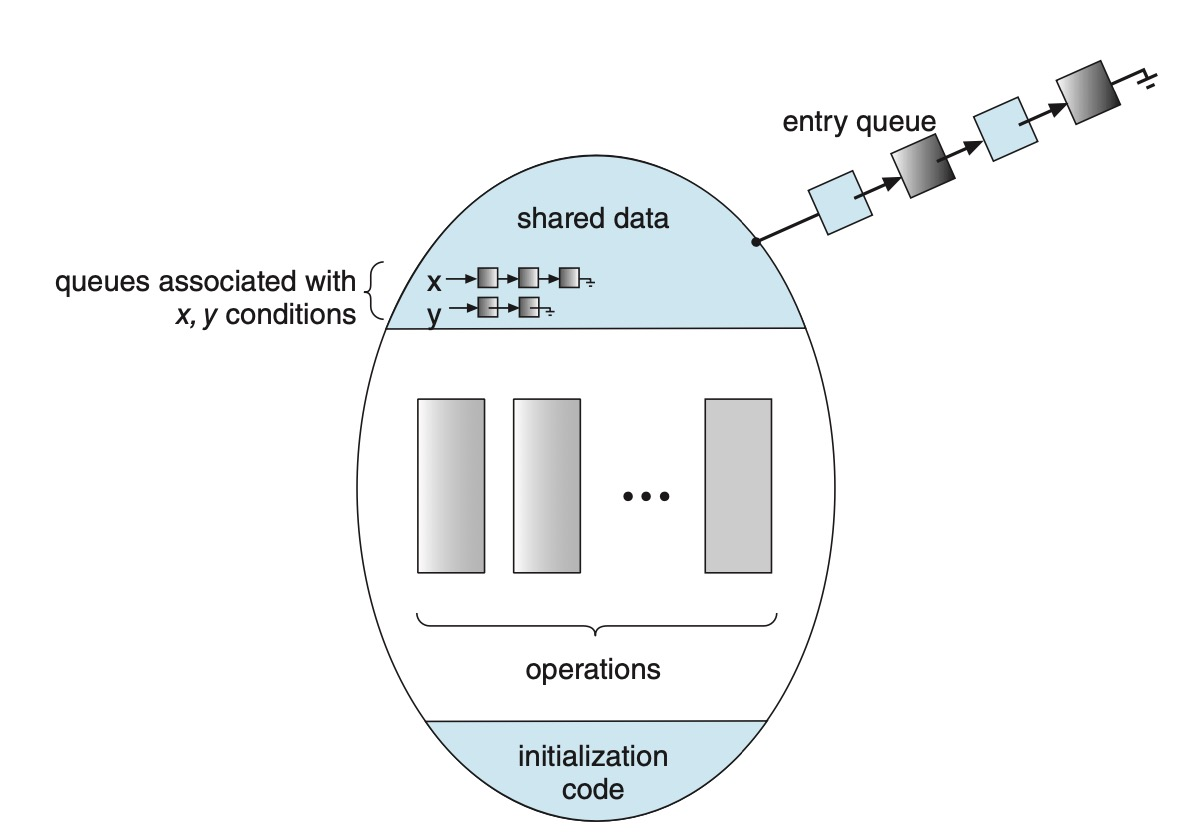
\includegraphics[width=0.6\linewidth]{assets/monitor.jpg}
    \caption{Monitor con variabili condition}
\end{figure}

\subsection{Gestione di signal}
Quando un processo $P$ invoca \texttt{signal()} su una risorsa che è attesa da un altro processo $Q$ si ottiene una situazione che può essere gestita in due modi:
\begin{sitemize}
    \item \textbf{Segnalare e attendere:} Il processo $P$, dopo la chiamata a \texttt{signal} esce dal monitor e lascia che $Q$ esegua la sua parte di codice.
    \item \textbf{Segnalare e procedere:} Il processo $P$ completa la sua esecuzione e poi $Q$ viene eseguito.
\end{sitemize}

\spacer
La seconda opzione, segnalare e procedere, sembra essere più ragionevole finché non si considera che la condizione che $P$ segnala potrebbe non essere più valida quando $Q$ arriva ad essere eseguito.
